\documentclass[reprint, nobibnotes, amssymb, amsmath, amsfonts, physics, mathtools, mathrsfs, floatfix]{revtex4-1}
\usepackage{graphicx}
\usepackage[english]{babel}


\newcommand{\redchi}{$\tilde{\chi}^2\,$}

\begin{document}

  \title{Relativistic Dispersion of Free Electrons}

  \author{Aman LaChapelle}
  \affiliation{The University of Chicago}


  \begin{abstract}
    We use a high-purity Germanium detector to measure with high precision the energies of incoming photons in the radiation spectrum.  We measure the kinetic energy of electrons from which these incoming photons scatter to determine the relativistic limit of the electronic dispersion relation in Ge crystal.  We determine that the well known special relativistic energy-momentum relation holds with remarkable accuracy, the model returning values of $\frac{m}{m_e} = 0.9696 \pm 0.0007$ and $2B = 1.019 \pm 0.001$.  B is the linear slope parameter that we use to characterize the relativistic mass, $\frac{p^2c^2}{2T} = BT + C$.  We finally examine the velocity and plot the dispersion relation of the electron moving with nontrivial fractions of $c$ in a Ge crystal.
  \end{abstract}

  \maketitle
  \newpage

  \section{Introduction and Theory}
    The goal we seek here is to verify the relativistic dispersion relation.  In general, we can reasonably take the dispersion relation to be the nearly free electron model, especially in the case of relativistic electrons.  When the kinetic energy of an electron is such that its velocity exceeds trivial fractions of $c$, the free electron approximation works exceedingly well as a basic picture of the band structure.  Thus, we are measuring the linear part of the electron's dispersion relation in order to determine the coefficients.  In essence, as the electron moves faster, we see the band flatten into a line from the parabolic structure that we expect from a typical electron.  In performing the detection, we make use of a high-purity Germanium crystal whose electrons are tightly bound - reducing the probability of electron-electron interactions once we knock an electron from its tethering with a high-energy photon.

    \hspace{.25cm}

    The electron energy after a high-energy scattering is given by the Compton Edge - this feature represents the energy of a photon that has undergone scattering with an electron with an angle of $\pi$ exactly once.  We can determine the momentum of the electron given this information because the energy deposited by the photon will be exactly the excess energy given to the electron.  Furthermore, we know that since Germanium has, to a good approximation, a tight-binding band structure, the electron will be both (mostly) stationary - in that it is tightly bound to its lattice site, and that once we excite it there will be a small probability of collision.~\cite{germanium_structure}  One interesting consequence of exciting an electron forcibly this way is that we will see a new hole in the Ge structure until the electron deposits its energy and drops back into the valence band, causing changes in the conductivity of Ge for a short time.

    \hspace{.25cm}

    We are not, however, concerned with the conductivity of the Ge crystal (aside from measurement of charge movement), we are concerned with the photon energies scattered off electrons as well as the direct incoming photon energies.  We will use energy spectra that represent the detector's response to these photons.

    \begin{figure}[h]
      \centering
      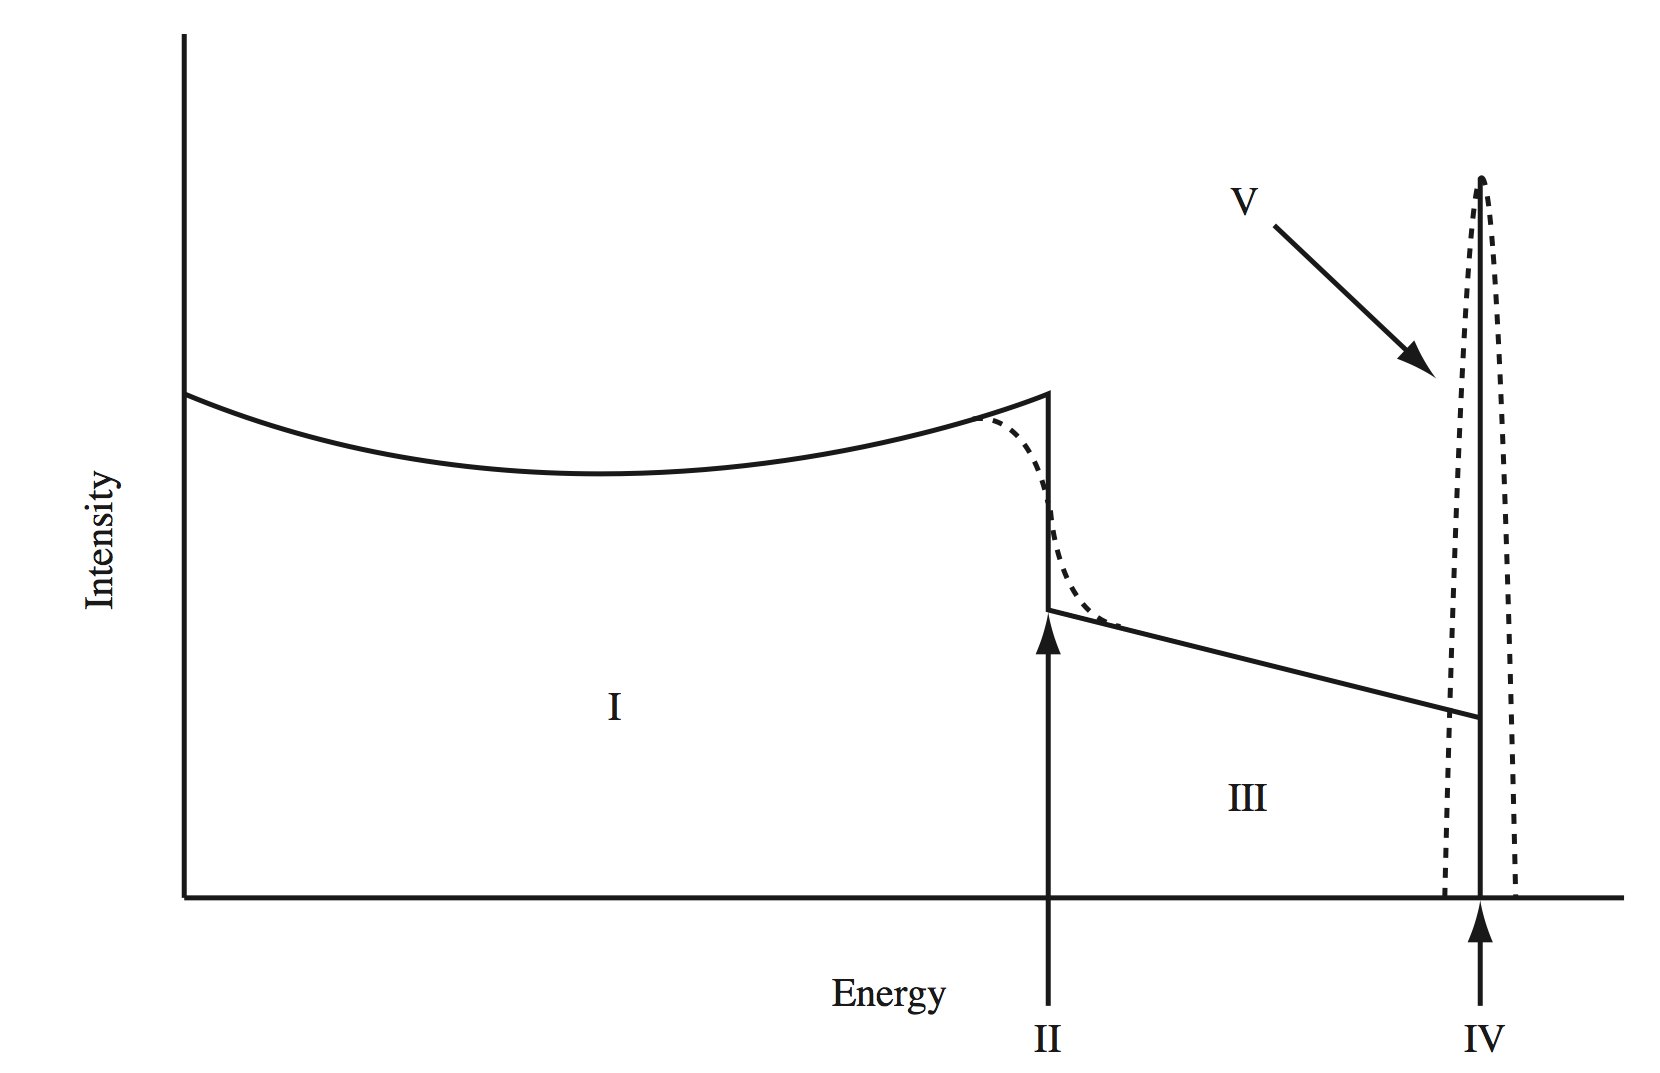
\includegraphics[width=\linewidth]{energy_spectrum.png}
      \caption{We are mainly concerned with features II and IV - these will tell us the electron energy after the compton scattering (indirectly via photon energy) and the direct incoming photon energy, respectively.~\cite{lab_manual} \label{fig:labeled_spectrum}}
    \end{figure}

    In order to find the electrons' momentum from a detector that is very sensitive to energy, we will use conservation of energy in order to show that we can extract the electron's kinetic energy from the photon energies after scattering once and the photon direct incoming energy.  We start by realizing that the photon energy at the full peak is equal to the energy of the photon after scattering plus the kinetic energy imparted to the electron, giving us the following relations.

    \begin{gather}
      E_\gamma = E_\gamma ' + T \\
      \text{Turning this into momentum using the photon dispersion $E = pc$}\nonumber\\
      \frac{E_\gamma}{c} = p - \frac{E_\gamma '}{c} \\
      \text{Therefore we have for the electron momentum}\nonumber\\
      pc = 2E_\gamma - T
    \end{gather}

    Now that we have the electron's momentum after a scattering event, we will be able to determine its dispersion relation using quantities that we can measure, namely, $E_\gamma$ and $T$.

    \hspace{.25cm}

    In order to 'discover' the special relativistic dispersion relation, we will plot the classical non-relativistic mass and see that it changes as a function of energy.  Namely, we take the following to be true:

    \begin{gather}
      T = \frac{p^2}{2m_e} \\
      \frac{p^2c^2}{2T} = m_ec^2
    \end{gather}

    or so we would hope.  We will see that this is not, in fact, constant as we would expect and thus we will find that the actual relation is something more like the following:

    \begin{gather}
      \frac{p^2c^2}{2T} = BT + C \label{eq:fitfn} \\
      B = 1/2 \\
      C = m_ec^2 \\
      \text{which would imply the following:}\nonumber \\
      p^2c^2 = 2m_ec^2 T + T^2
    \end{gather}

    which is the well-known relativistic dispersion relation.  We can see that in the limit where $T << 2m_ec^2$ we recover the classical relation where $\frac{p^2}{2T}$ reduces to the electron rest mass.  As a further bonus, when we take the same limit we can also see that the classical quadratic dispersion is recovered as well - $T = \frac{p^2}{2m}$.

    \hspace{.25cm}

    Now that we have established the relativistic form of the dispersion relation, we will explore its consequences.  The first thing that we can do is to calculate and compare the electron's rest mass as follows:
    \begin{equation}
      m_ec^2 = \frac{2E_\gamma(E_\gamma - T)}{T} \label{eq:rest_mass}
    \end{equation}

    Another quantity of interest is the velocity of the electron.  We can show that the following holds ($c = 1$):
    \begin{equation}
      v = \frac{T(2E_\gamma - T)}{T^2 - 2E_\gamma T + 2E_\gamma^2} \label{eq:velocity}
    \end{equation}

    Previously we have been using the dispersion relation implicitly to understand the electron dynamics of the system.  What we will now do, is to actually plot the dispersion relation, E vs p and get an idea of the relativistic region of the band structure in Ge.  The form this takes is as follows:
    \begin{equation}
      T = \sqrt{(m_ec^2)^2 + p^2c^2} - m_ec^2 \label{eq:dispersion}
    \end{equation}

  \section{Experimental Methods}
    Taking data is extremely simple in this case.  We have a simple Ge crystal that is immersed in $LN_2$.  We then place a radioactive button source directly in front of it using a small holder, and we simply wait for counts to accumulate on the PHA.

    \hspace{.25cm}

    We use 6 sources - Na-22, Co-57, Ba-133, Cs-137, Bi-207, and In-116.  In order to use the last source, we have to insert the foil plates into the high-energy neutron howitzer to turn the In-115 into In-116 by bombarding it with extremely high-energy neutrons.  Na-22 has two, very well-defined photon peaks, at 511 keV and 1.2745 MeV.  Cs-137 also has a very well-defined peak, at 662 keV.  These three peaks are very easy to identify and have nice clean compton edges as well.  We will thus be using these for calibration and for our data.  This may seem to be irrational, however the rationale is thus: these peaks are easy to find and fit - since they are easy to fit they will provide 3 very stable and low-uncertainty points on the calibration curve.  We of course add other peaks that do not have well-defined compton edges as calibration peaks as well, and we end up having 7 points on our calibration curve.

    \hspace{.25cm}

    When a photon enters the crystal, we will see an electron scatter from its lattice site and be excited into the conduction band.  We then apply high voltage across the crystal to separate the electron and hole and count the charge.  This counting is done by a charge-sensitive pre-amplifier which produces pulses with height that is proportional to the amount of charge (and the energy of the photon/the number of electrons it scattered).  The pulses are sent through an amplifier to the Pulse Height Analyzer (PHA), which bins the data and produces the histogram we are used to seeing, as in Figure~\ref{fig:labeled_spectrum}.  In this way, the detector provides information about the kinetic energy of the scattered electron, and by inference the recoil energy of the photon.  The full energy peak of course refers to photons that enter the detector and deposit all their energy in the crystal.  We thus have all the quantities of interest, $E_\gamma$, $E_\gamma'$, and $T$.

    \subsection{Calibration}
      The PHA returns counts vs. channel.  Because we need the axis in units of energy, we must perform a calibration.  In order to do this, we identify peaks that don't have well-defined compton peaks and use their positions and known energies in order to calibrate the channel axis to energy.  We know that the energy is related to the channel linearly, and we can therefore write the following:
      \begin{gather}
        E = A \cdot ch + B \label{eq:calibration}\\
        \text{Inverting this,}\nonumber \\
        ch = A'E + B' \\
        A = 1/A' \\
        B = -B'/A'
      \end{gather}

      using Eq.~\ref{eq:calibration}, we will then be able to convert the channel axis to energy.  The most important piece of information we gain from this procedure is the calibration itself.  The second most important information is the fact that the uncertainty in the compton edge dominates over the uncertainty in the peak locations, which informs future decisions about error analysis.

  \section{Discussion and Analysis}
    \subsection{Calibration}
      The first step in performing our analysis is calibrating our instrumentation.  Thus, we perform a linear fit to extract the parameters by which the energy is related to a PHA channel.  Results are summarized in Figure~\ref{fig:calibration}.

      \begin{widetext}

        \begin{figure}[h]
          \centering
          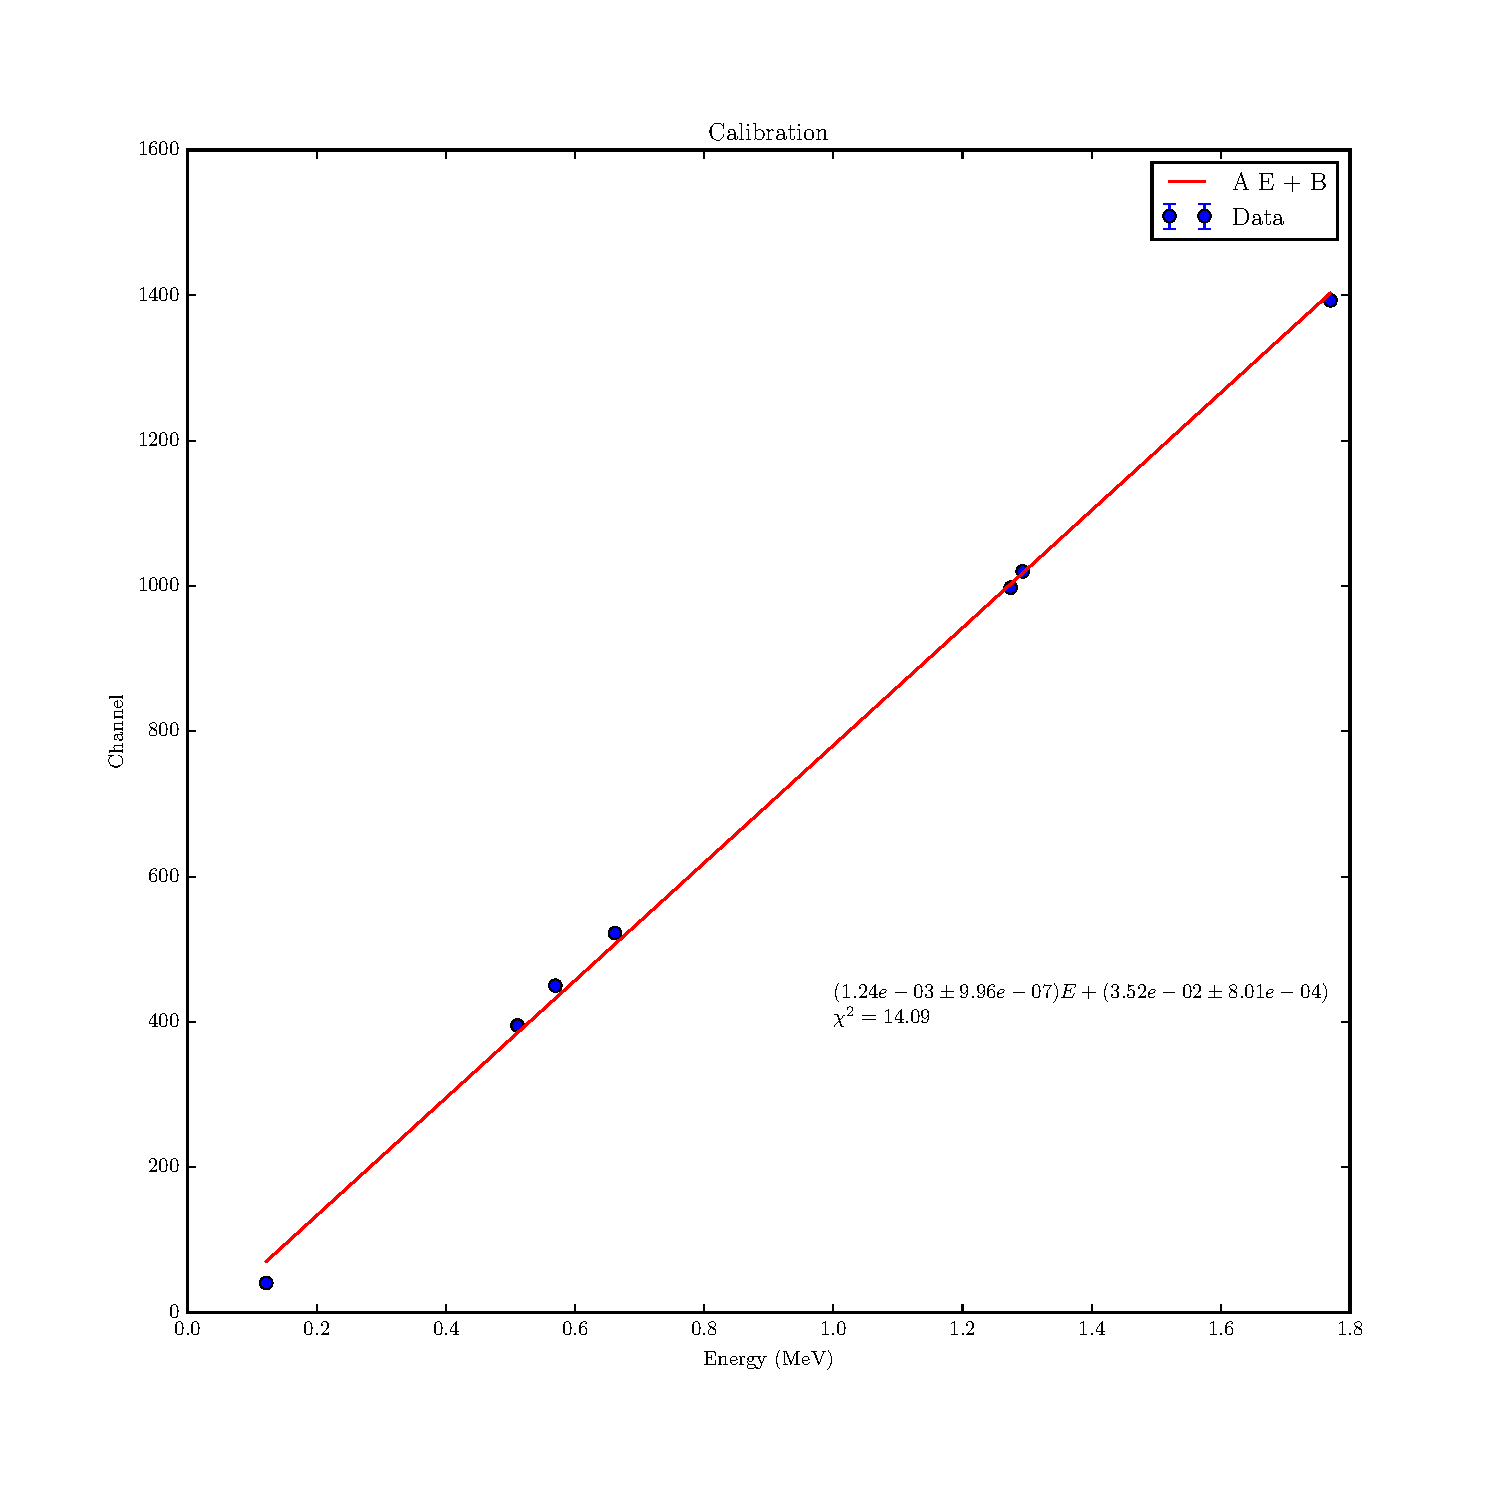
\includegraphics[width=\linewidth]{../plots/calibration.pdf}
          \caption{The point uncertainties are extraordinarily low because we are using full-energy peaks to get these points.  This means that they can be determined to around 1 channel, and as such uncertainties will be very small. \label{fig:calibration}}
        \end{figure}

      \end{widetext}

      The energy peaks we used were the following:

      \begin{table}[h]
        \centering
        \begin{tabular}{|c|c|c|}
          \hline
          Element & Channel ($\pm1$ channel) & Energy (exact) \\ \hline
          Co-57 & 45 & .122 MeV \\ \hline
          Na-22 & 394 & .511 MeV \\ \hline
          Bi-207 & 450 & .5696 MeV \\ \hline
          Cs-137 & 522 & .662 MeV \\ \hline
          Na-22 & 997 & 1.2745 MeV \\ \hline
          In-116 & 1019 & 1.2933 MeV \\ \hline
          Bi-207 & 1393 & 1.7697 MeV \\ \hline
        \end{tabular}
        \caption{Correspondence between element, channel and full energy capture peaks. \label{tab:calibration_points}}
      \end{table}

      In order to propagate uncertainties forward, we took a normal distribution around each point and simulated 1000 data sets where each point was drawn from this normal distribution at random.  The fit uncertainties reflect the standard deviation of that fit parameter after performing this check.

    \subsection{Feature Identification}
      The first step in identifying our features is to simply plot the spectra for each element and point out features we will be using later.  We will begin with Cs-137 since its spectrum is the simplest and work our way up.  We will notice that some sources didn't give any noticeable compton edges, and only contributed peaks.  These peaks were mainly used for calibration - we had no real use for peaks that don't have identifiable compton edges.  The observant reader will also notice that our calibration curve doesn't include the second Co-57 peak.  This is because we weren't sure what the feature just below it in energy was, and whether it was a peak or compton edge, or possibly even vice-versa (though that seemed unlikely).  Mostly, we are unsure of what that feature is and labeled it as a full energy peak because it most likely is (and from the decay scheme it's where it should be), but in any case we were not confident in that peak and so left it out.

      \begin{widetext}

        \begin{figure}[h]
          \centering
          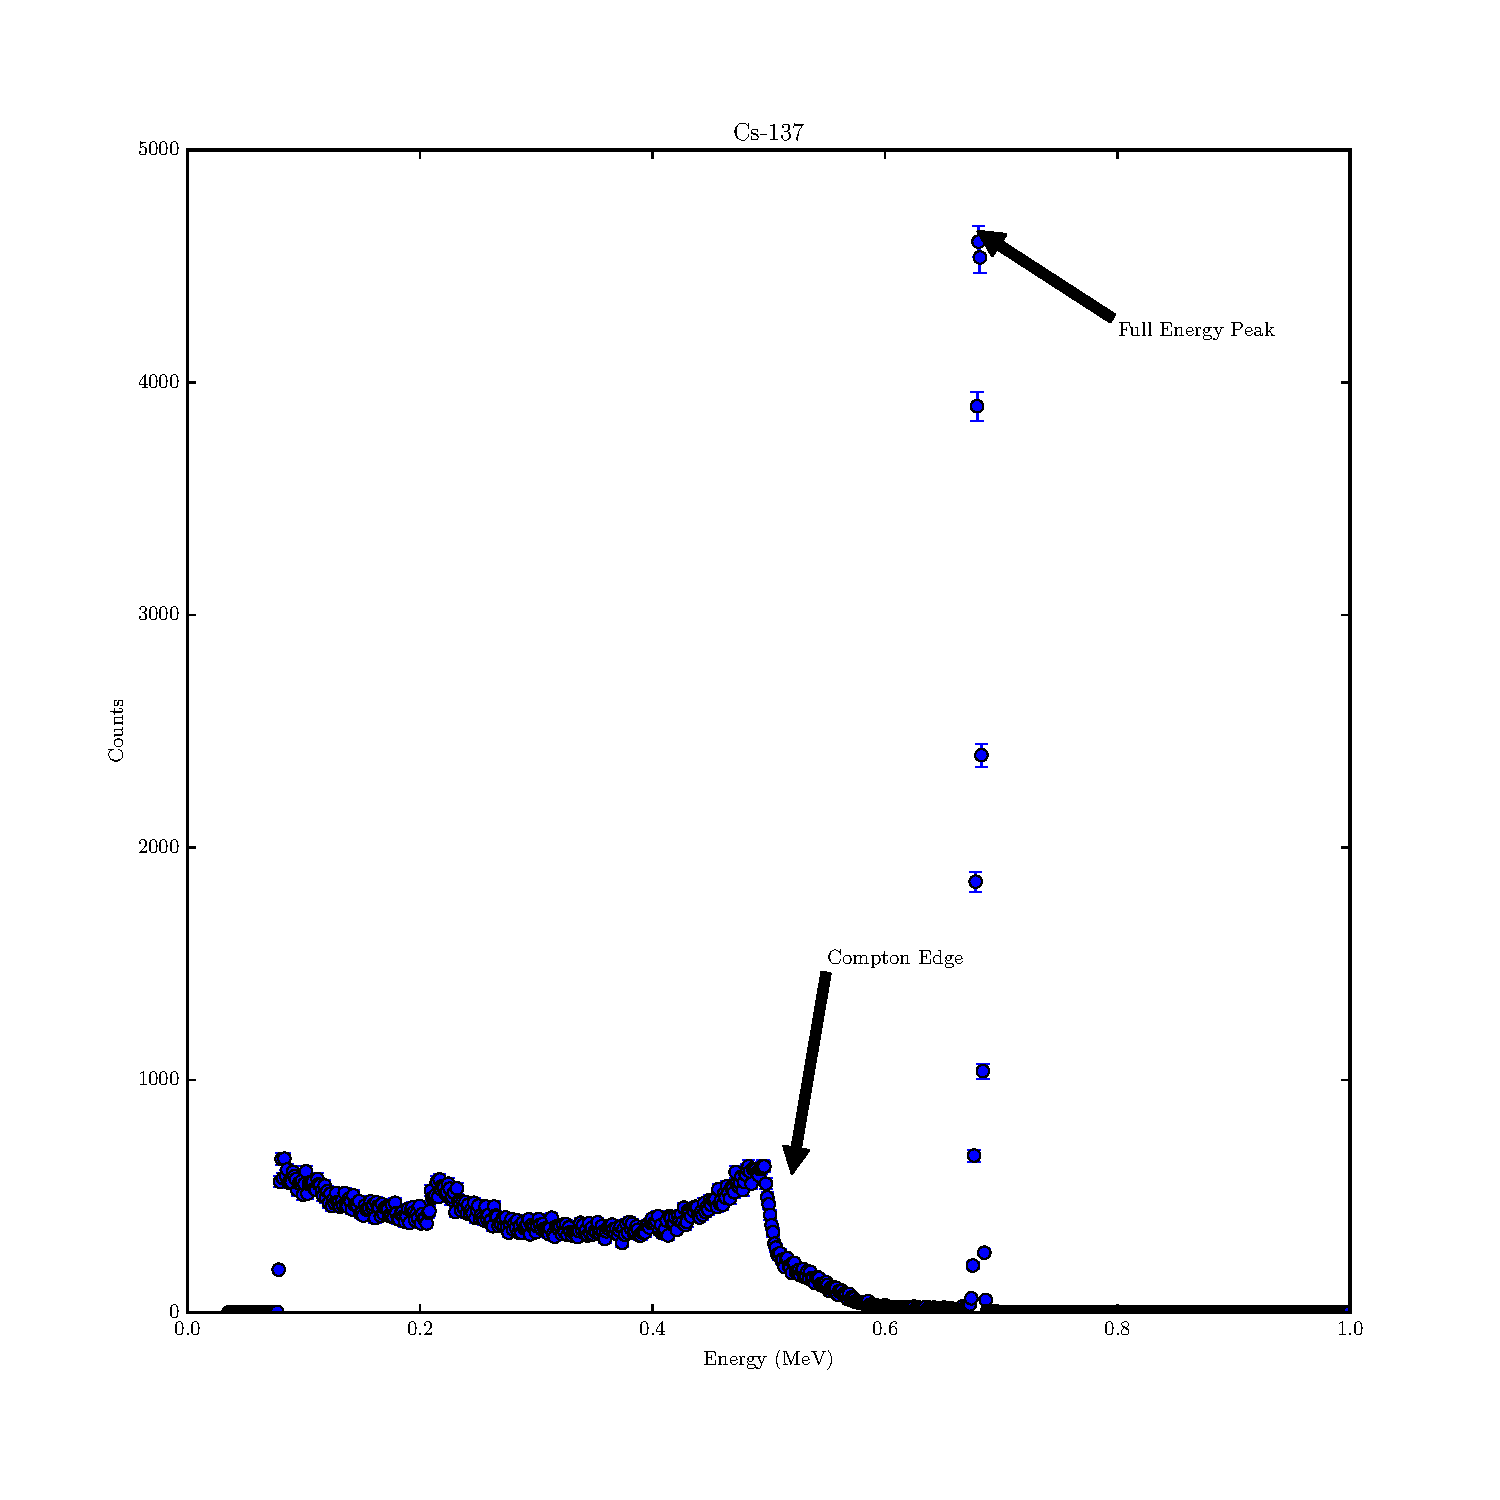
\includegraphics[width=\linewidth]{../plots/Cs-137.pdf}
          \caption{Cs-137 with full energy peak and Compton edge identified \label{fig:cs}}
        \end{figure}

        \begin{figure}[h]
          \centering
          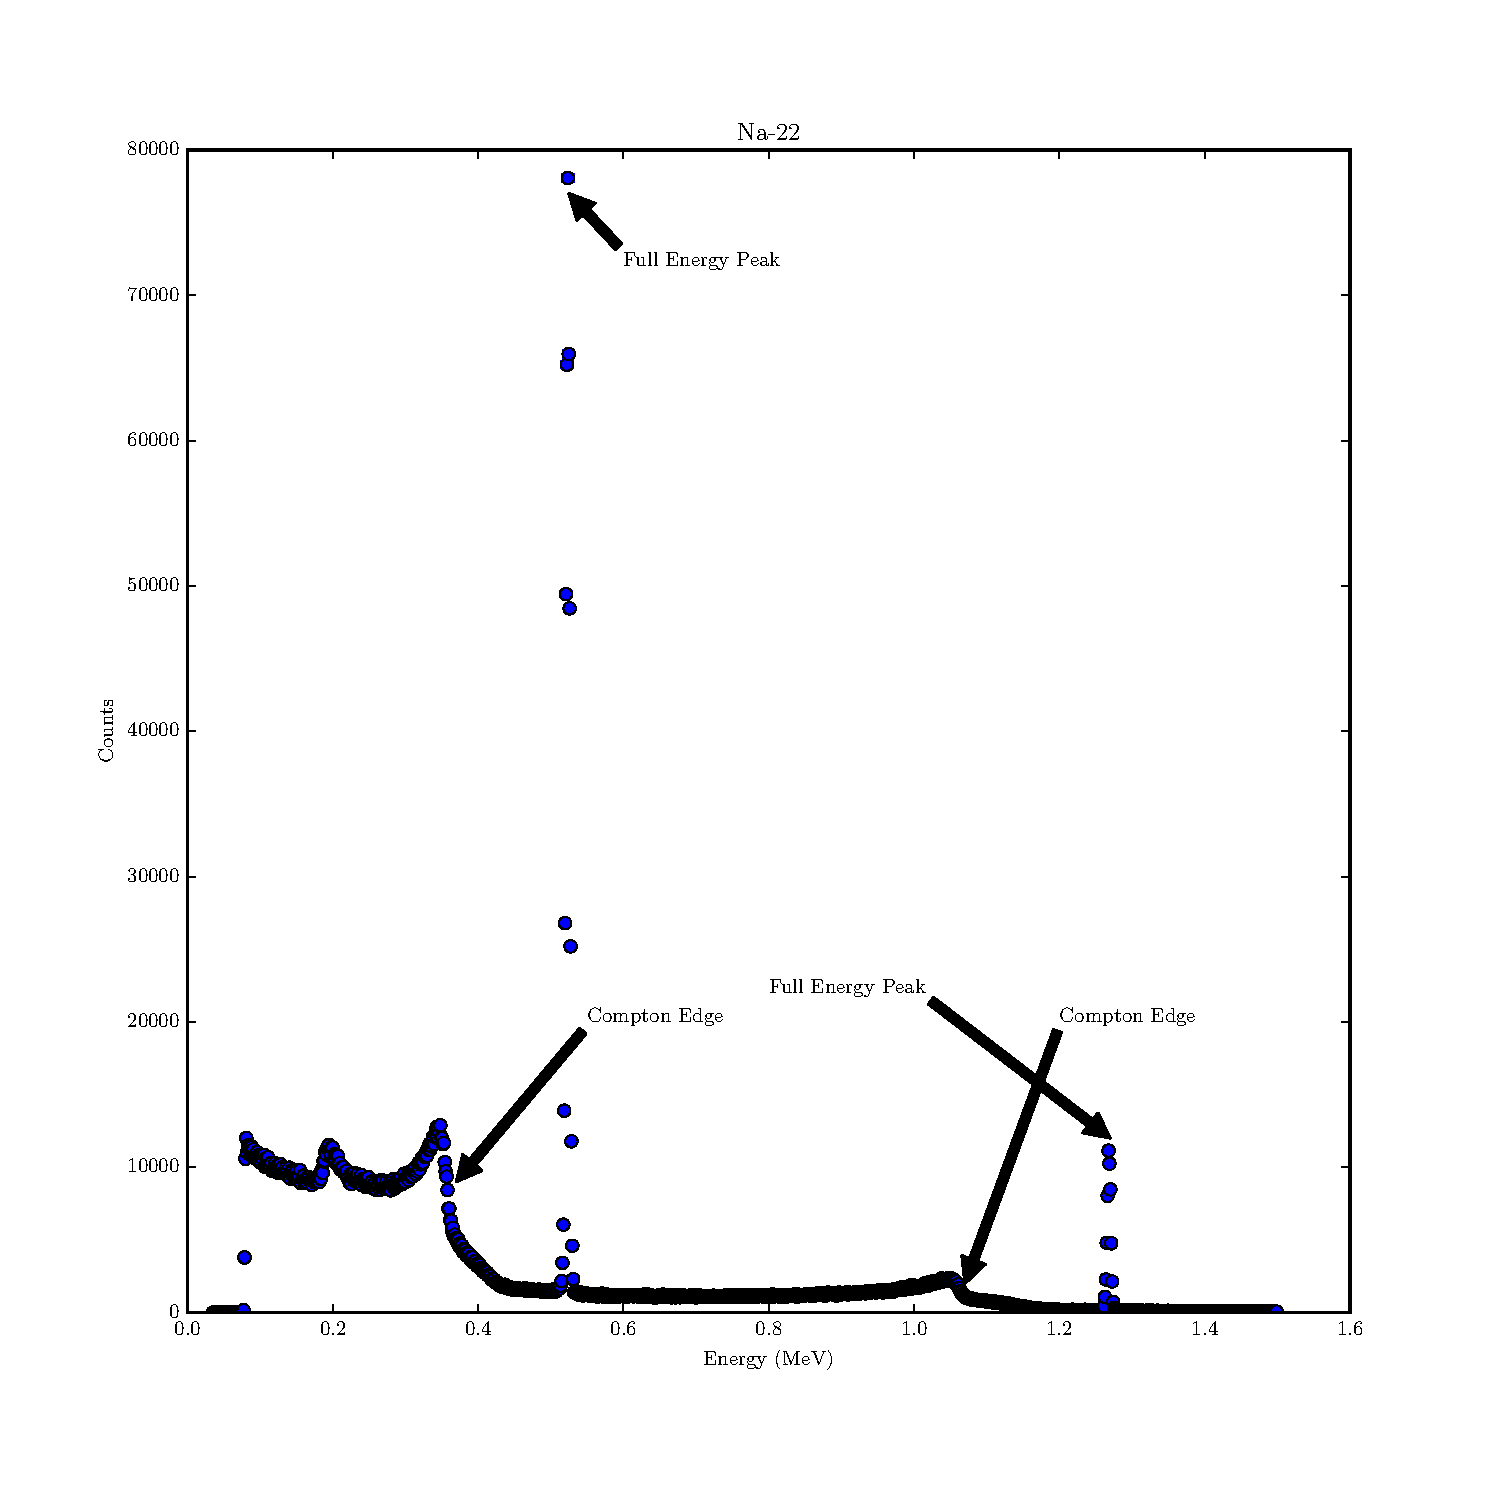
\includegraphics[width=\linewidth]{../plots/Na-22.pdf}
          \caption{Na-22 with full energy peaks and Compton edges identified \label{fig:na}}
        \end{figure}

        \begin{figure}[h]
          \centering
          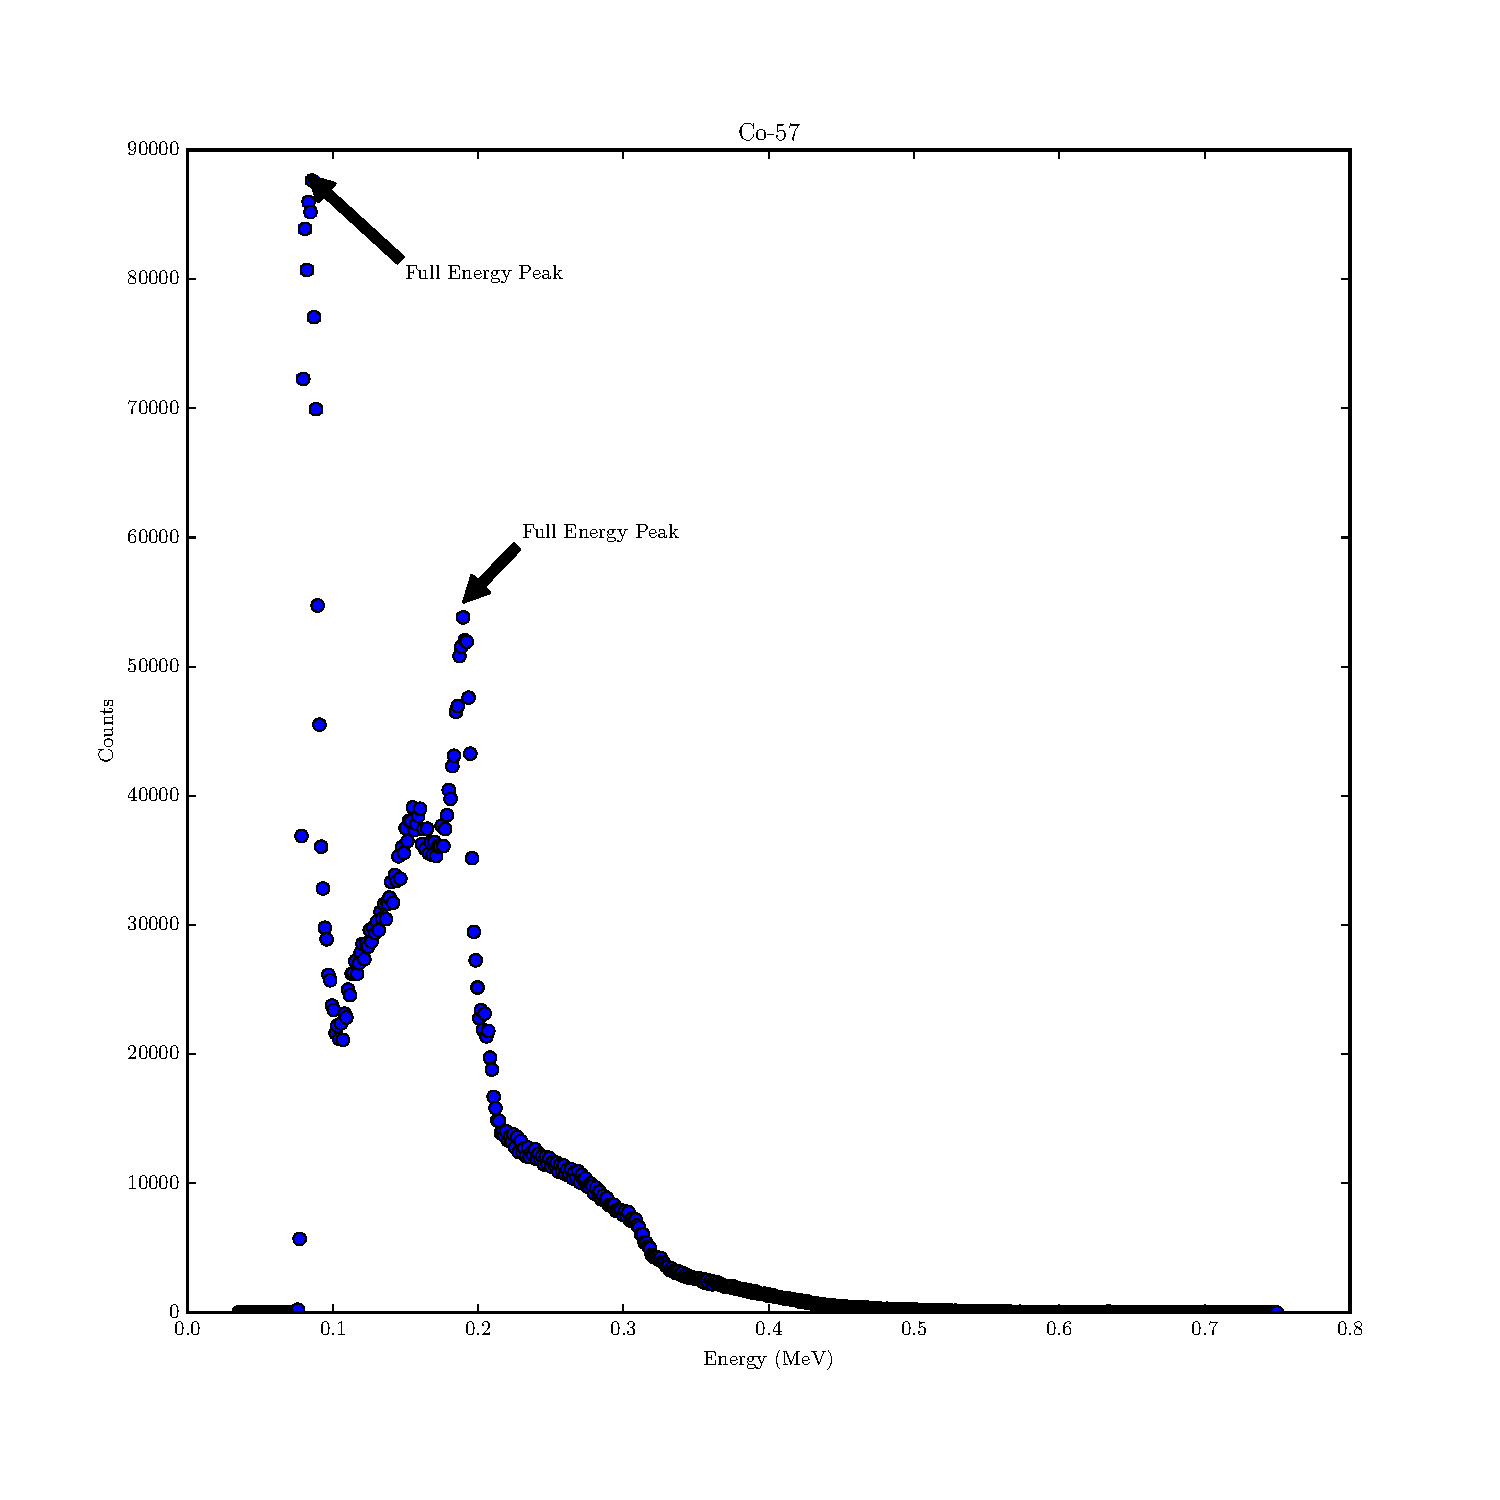
\includegraphics[width=\linewidth]{../plots/Co-57.pdf}
          \caption{Co-57 with full energy peaks identified \label{fig:co}}
        \end{figure}

        \begin{figure}[h]
          \centering
          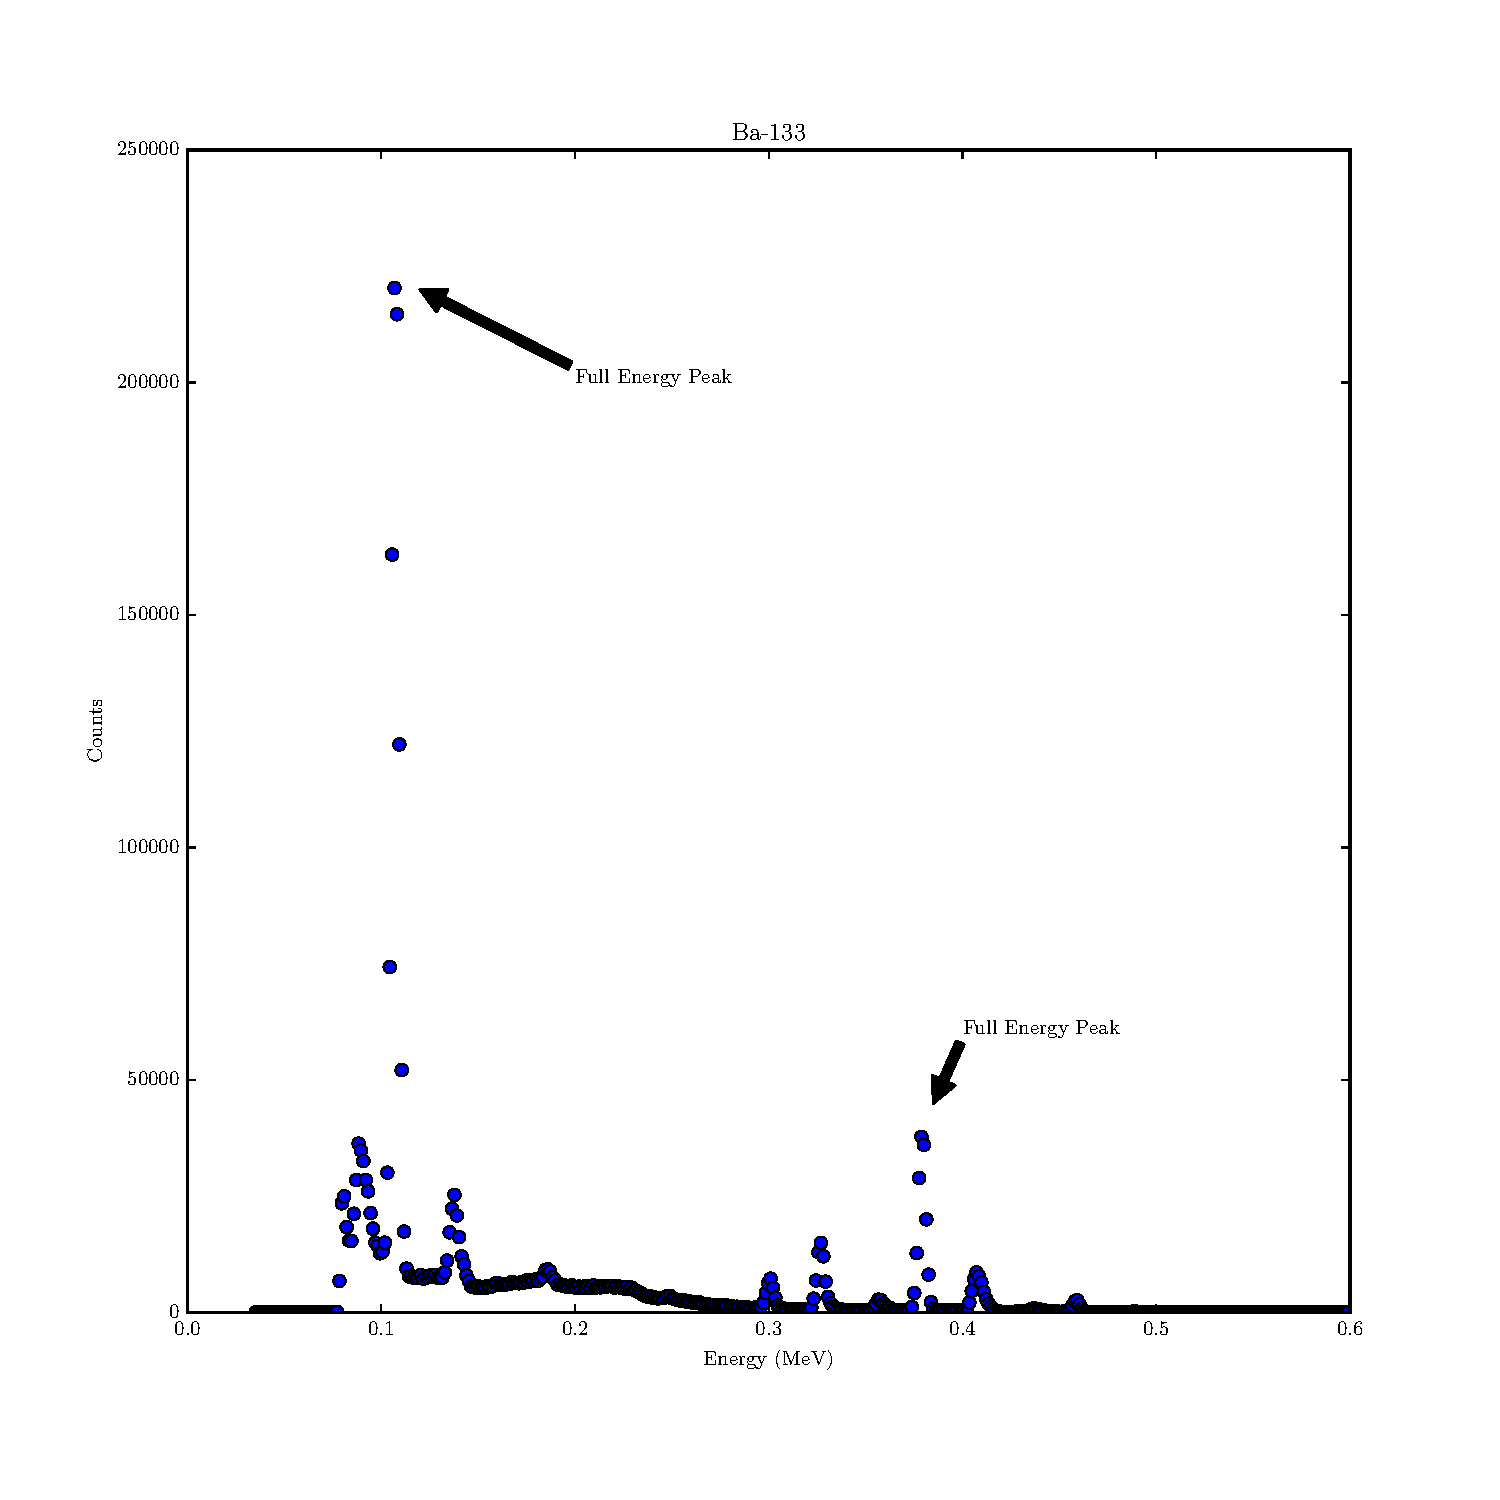
\includegraphics[width=\linewidth]{../plots/Ba-133.pdf}
          \caption{Ba-133 with full energy peaks identified \label{fig:ba}}
        \end{figure}

        \begin{figure}[h]
          \centering
          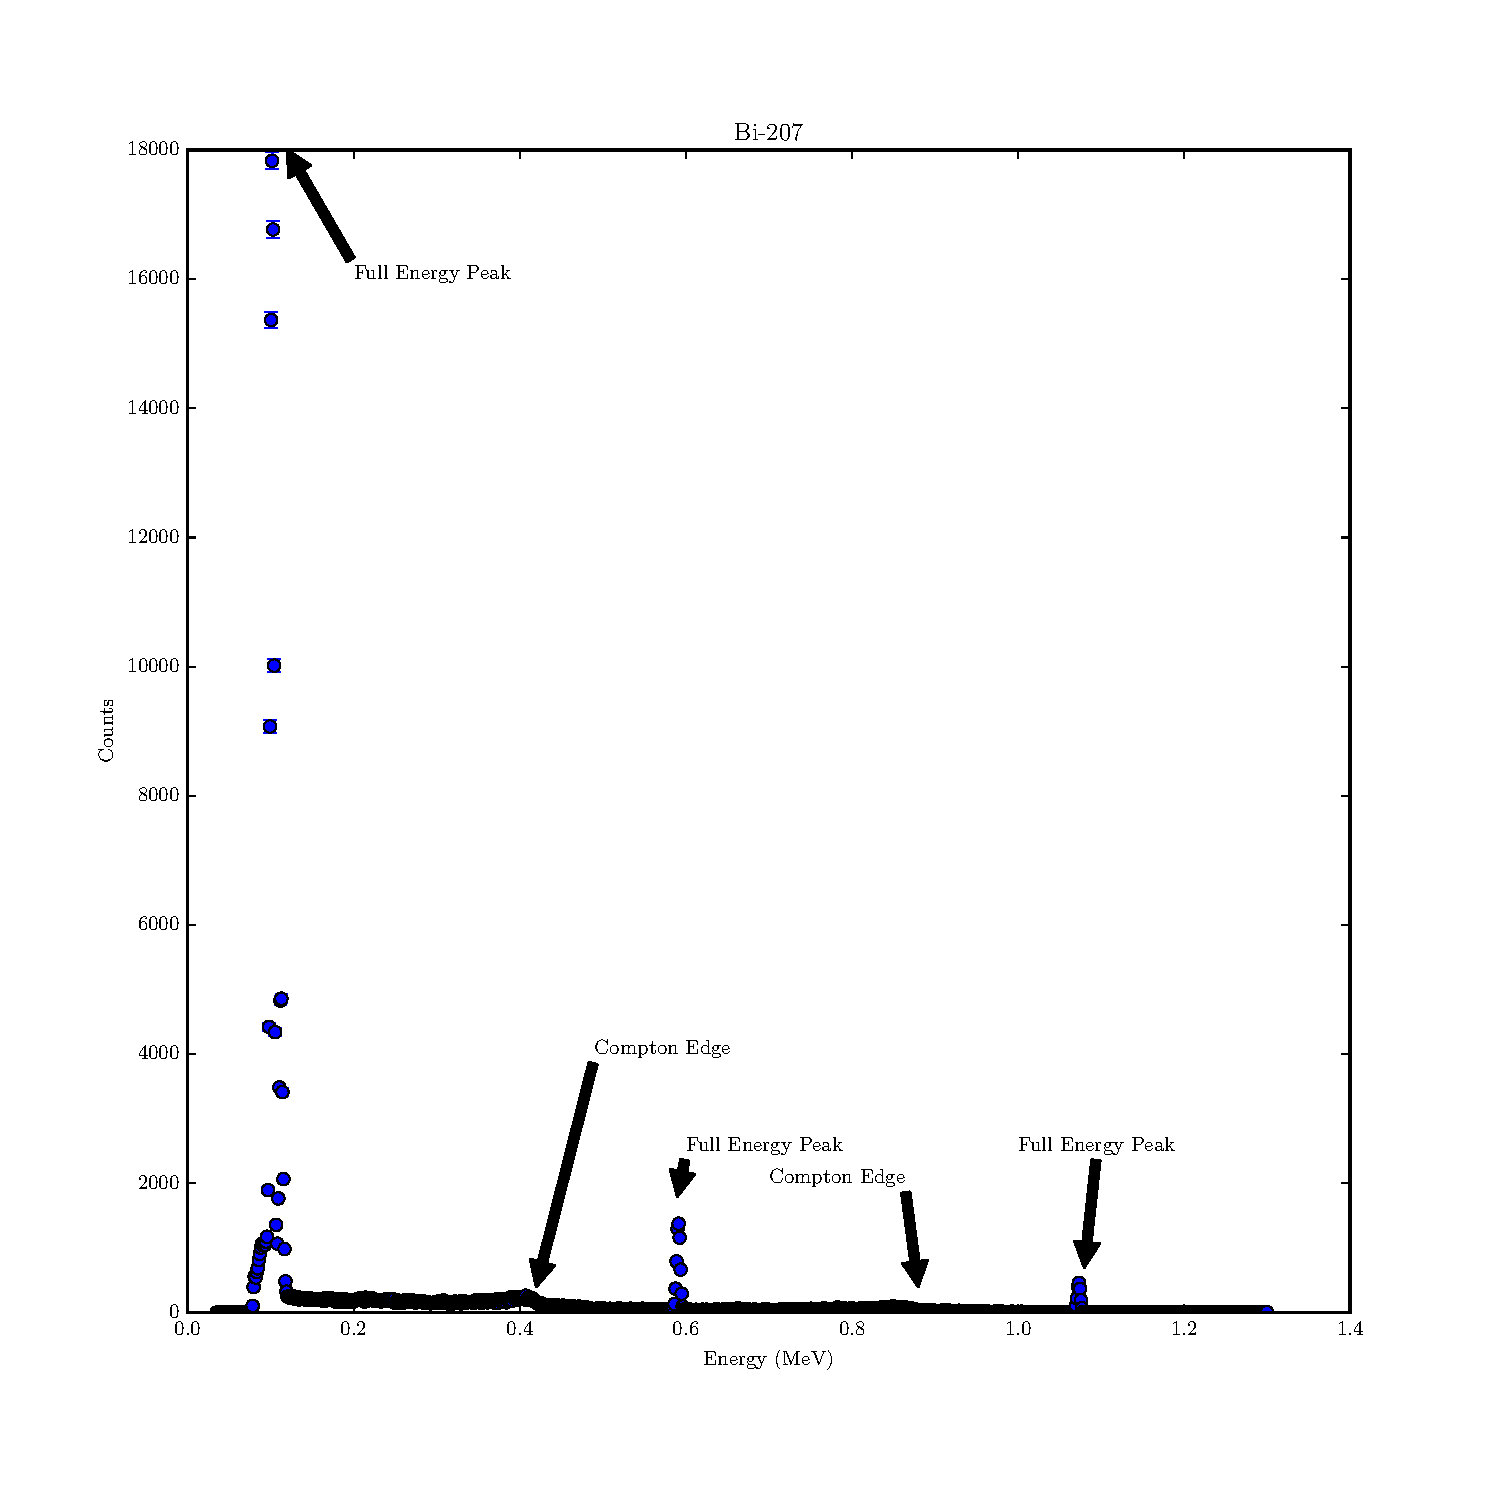
\includegraphics[width=\linewidth]{../plots/Bi-207.pdf}
          \caption{Bi-207 with full energy peaks and Compton edges identified \label{fig:bi}}
        \end{figure}

        \begin{figure}[h]
          \centering
          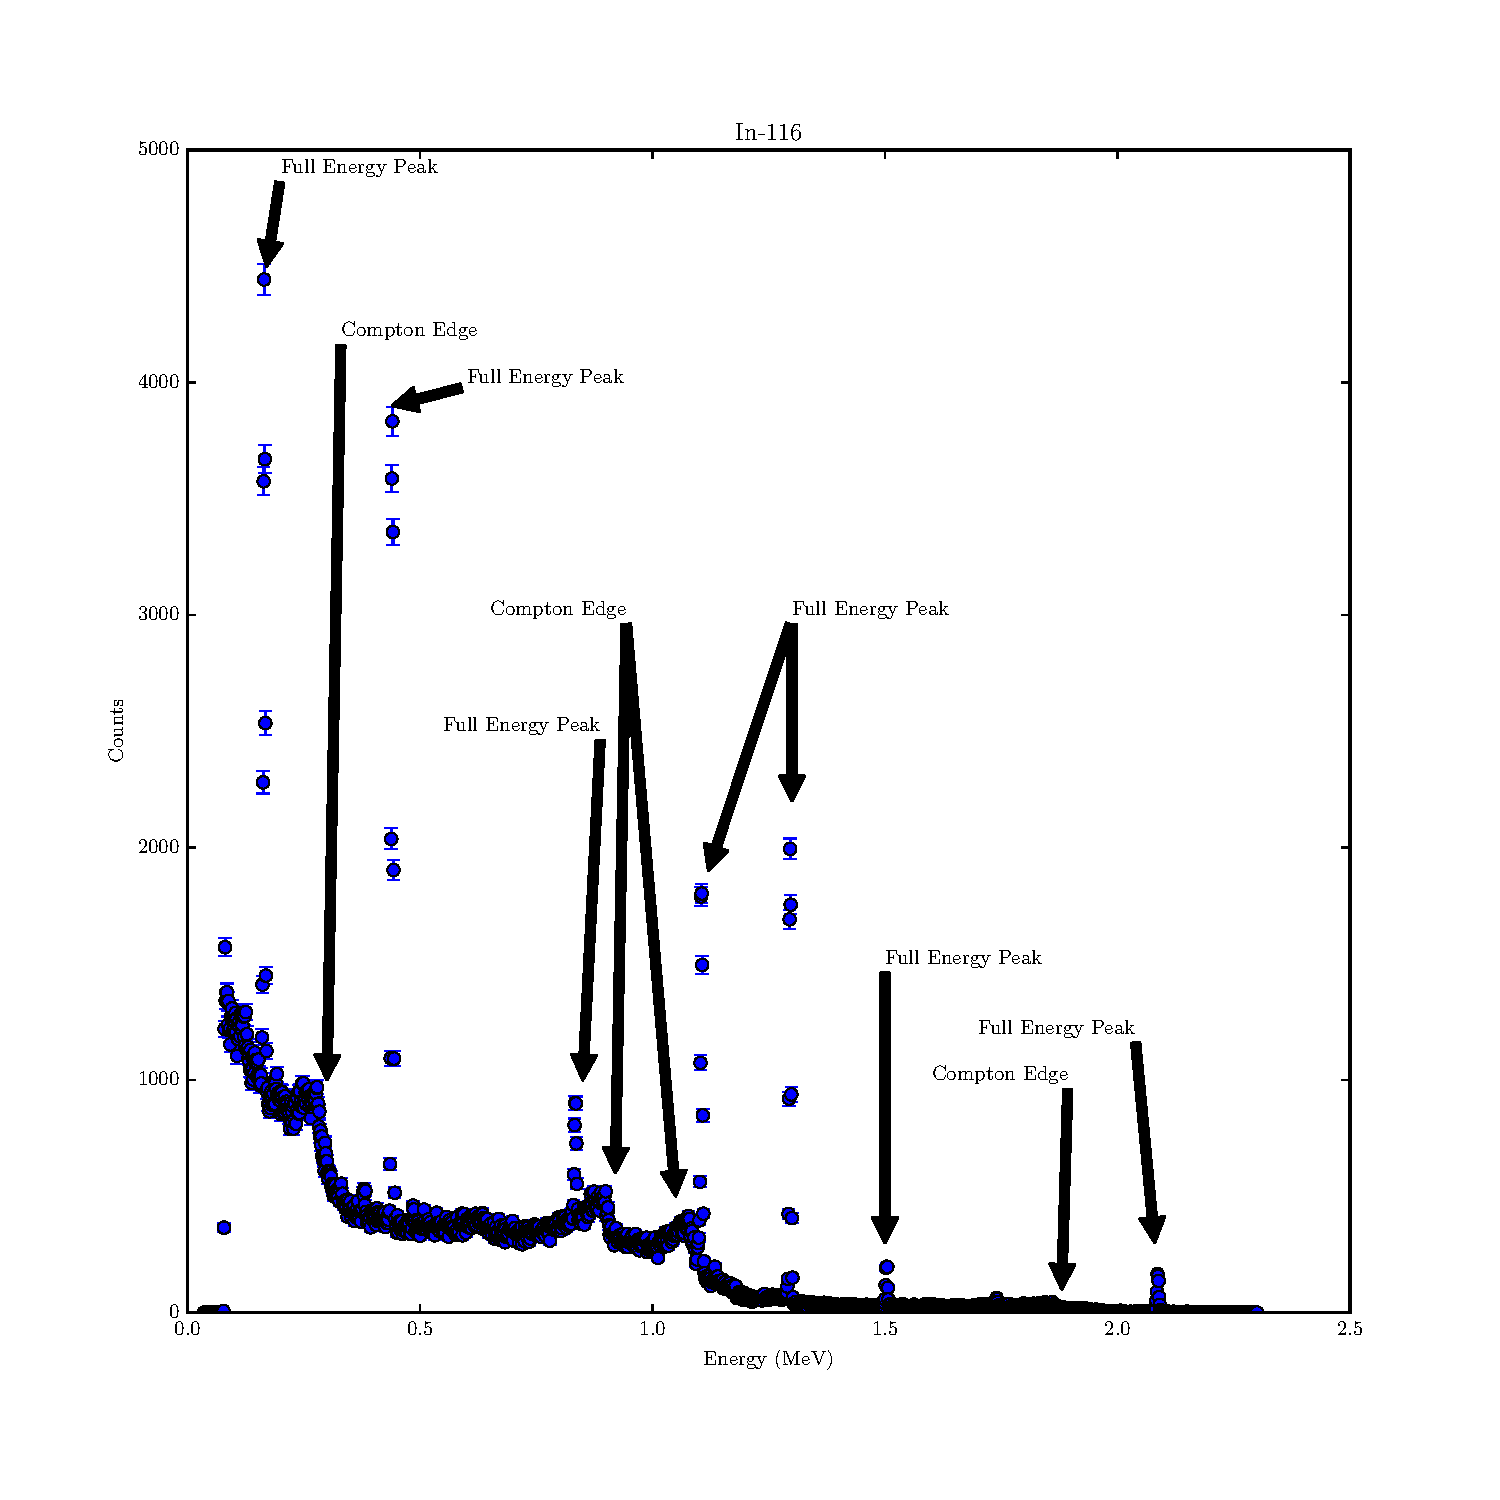
\includegraphics[width=\linewidth]{../plots/In-116.pdf}
          \caption{In-116 with full energy peaks and Compton edges identified \label{fig:in}}
        \end{figure}

      \end{widetext}

      In order to keep track of this madness, we have in order: Cs-137, Figure~\ref{fig:cs}; Na-22, Figure~\ref{fig:na}; Co-57, Figure~\ref{fig:co}; Ba-133, Figure~\ref{fig:ba}; Bi-207, Figure~\ref{fig:bi}; and In-116, Figure~\ref{fig:in}.

      \hspace{.25cm}

      Now, because there are such a huge volume of peaks, we have done the following.  We picked out all of the significant peaks by eye, but we need to be certain that the peaks are where we think they are, and be able to estimate uncertanties properly.  So, picking the best few peaks, we performed fits to determine the parameters of the peaks (center, width, etc.) and found that our by-eye estimation was quite accurate both in picking out the center and also in estimating uncertainty.  Thus, we can simply confirm that what we picked is correct enough to use.  For the reader's graphical pleasure, an excellent specimen, a lovely peak that took marvellously to the fitting routine, Figure~\ref{fig:fitted_in}.

      \begin{figure}[h]
        \centering
        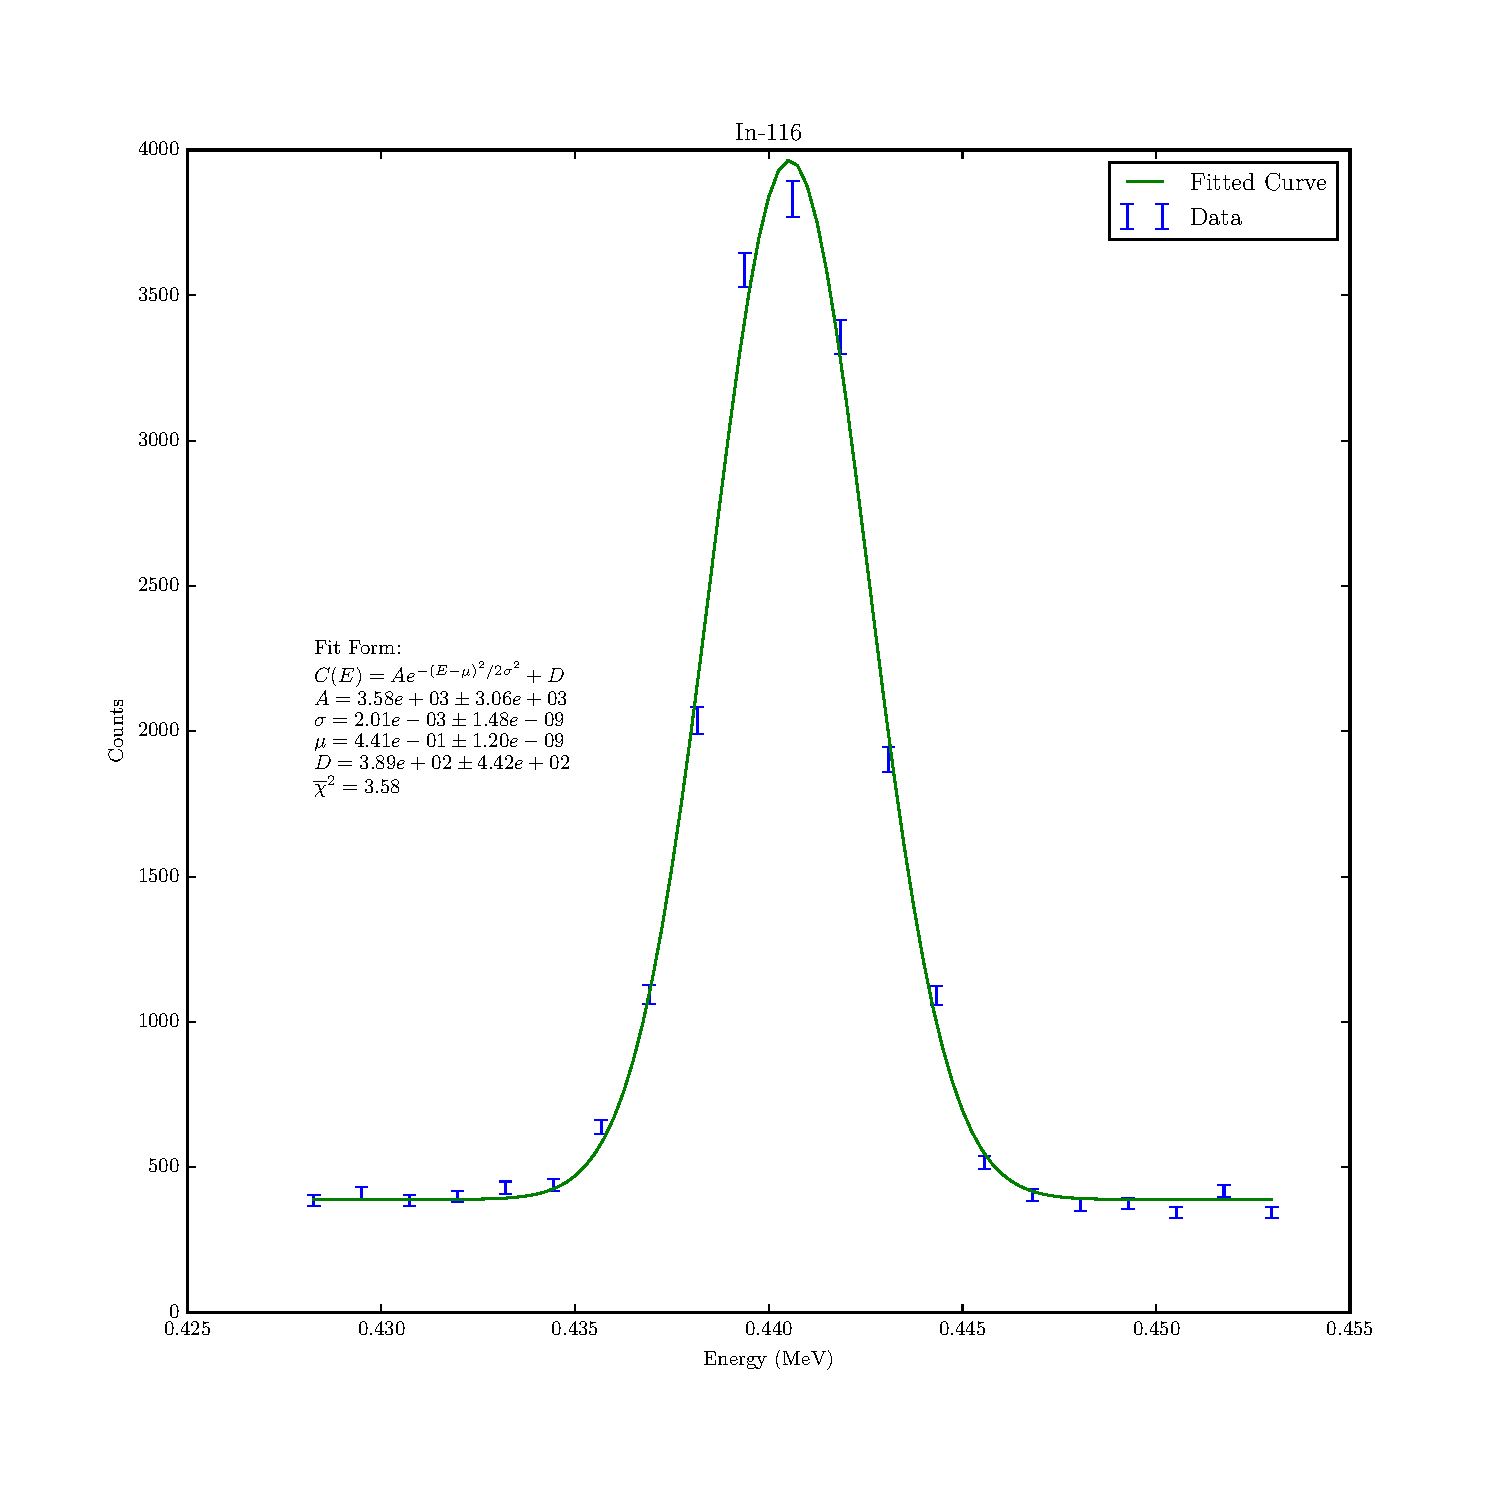
\includegraphics[width=\linewidth]{../plots/In-116_0_4405.pdf}
        \caption{One of the better examples of peaks, once fitted.  This confirms that our estimates for peak centers were accurate, and our estimation that the uncertainties were around 1 channel were also accurate. \label{fig:fitted_in}}
      \end{figure}

      % need to put table of peaks here along with status, etc





\bibliography{bib}
\bibliographystyle{plain}

\end{document}
